\chapter{Auswertung der Messdaten und Diskussion}
Im folgenden Kaptitel werden die im Experiment aufgenommenen Daten ausgewertet. 
Nach der Diskussion der Photolumineszenz und der 
Direktionalität, wird speziell auf die Temperaturabhängigkeit der 
Direktionalität eingegangen.
Dies wird gemacht um besser zu verstehen welche Rolle eine Temperaturänderung 
bei der direktionalen Lichtemission spielt.

\section{Photolumineszenz und Direktionalität bei konstanter Temperatur}~\label{sec:PL_u_Direktionalitaet}
Die gemessene Photolumineszenz (PL) der Probe (vgl. Abschnitt~\ref{sec:probe})
ist in Abbildung~\ref{fig:photo} als farblich dargestelle Intensitätsverteilung zu sehen. 
Die Temperatur (am Temperatursensor) hat zum Zeitpunkt der Messung $T = \SI{4}{\kelvin}$ betragen.
Der Graph der PL ist durch die Summation aller Einzelmessungen 
bei positiven und negativen Magnetfeld entstanden. 

Die Winkelachse in Abbildung~\ref{fig:photo} beschreibt den Winkelbereich unter welchen das 
emittierte Licht aus der Probe ausgetreten ist.
Die Wellenlängenachse charakterisiert die Energie die das emittierte Licht besitzt. 
Während der Durchführung des Experiments war das emittierte Licht als schwaches rotes Leuchten zu 
erkennen.
Die farblich dargestelle Intensität hat keine weiter spezifizierte physikalische Einheit, 
da es nur um Änderungen unter den Intensitäten geht. TODO wie normieren?
Der Winkelbereich wird auf $\theta = \pm \SI{20}{\degree}$ 
eingeschränkt um verzerrende Randeffekte/Artefakte zu vermeiden. 
Tatsächlich auflösbare wäre der Winkelbereich, aufgrund der numerischen Apertur, 
bei $\theta = \pm \SI{24}{\degree}$ 
(vgl. Abschnitt~\ref{sec:Beschreibung des Versuchsaufbaus}).

Wie in Abbildung~\ref{fig:photo} zu erkennen ist, ist die PL zentriert bei 
$\lambda = \SI{737}{\nano\meter}$ dargestellt. 
Das hat den Grund das dort genau das Maximum der PL liegt.
Die Energie des emittierten Lichts im Maximum beträgt $\SI{1,68}{\eV}$.
Eine Veranschaulichung des Maximums ist in Abbildung~\ref{fig:max} zu sehen.
Die Abnahme der Intensität an den Rändern der PL also unter ca. $\SI{735}{\nano\meter}$ und über ca. 
$\SI{740}{\nano\meter}$ bedeuten, 
dass die Probe ab diesem Wellenlängen fast bis kein Licht mehr emittiert.
\begin{figure}
    \centering
    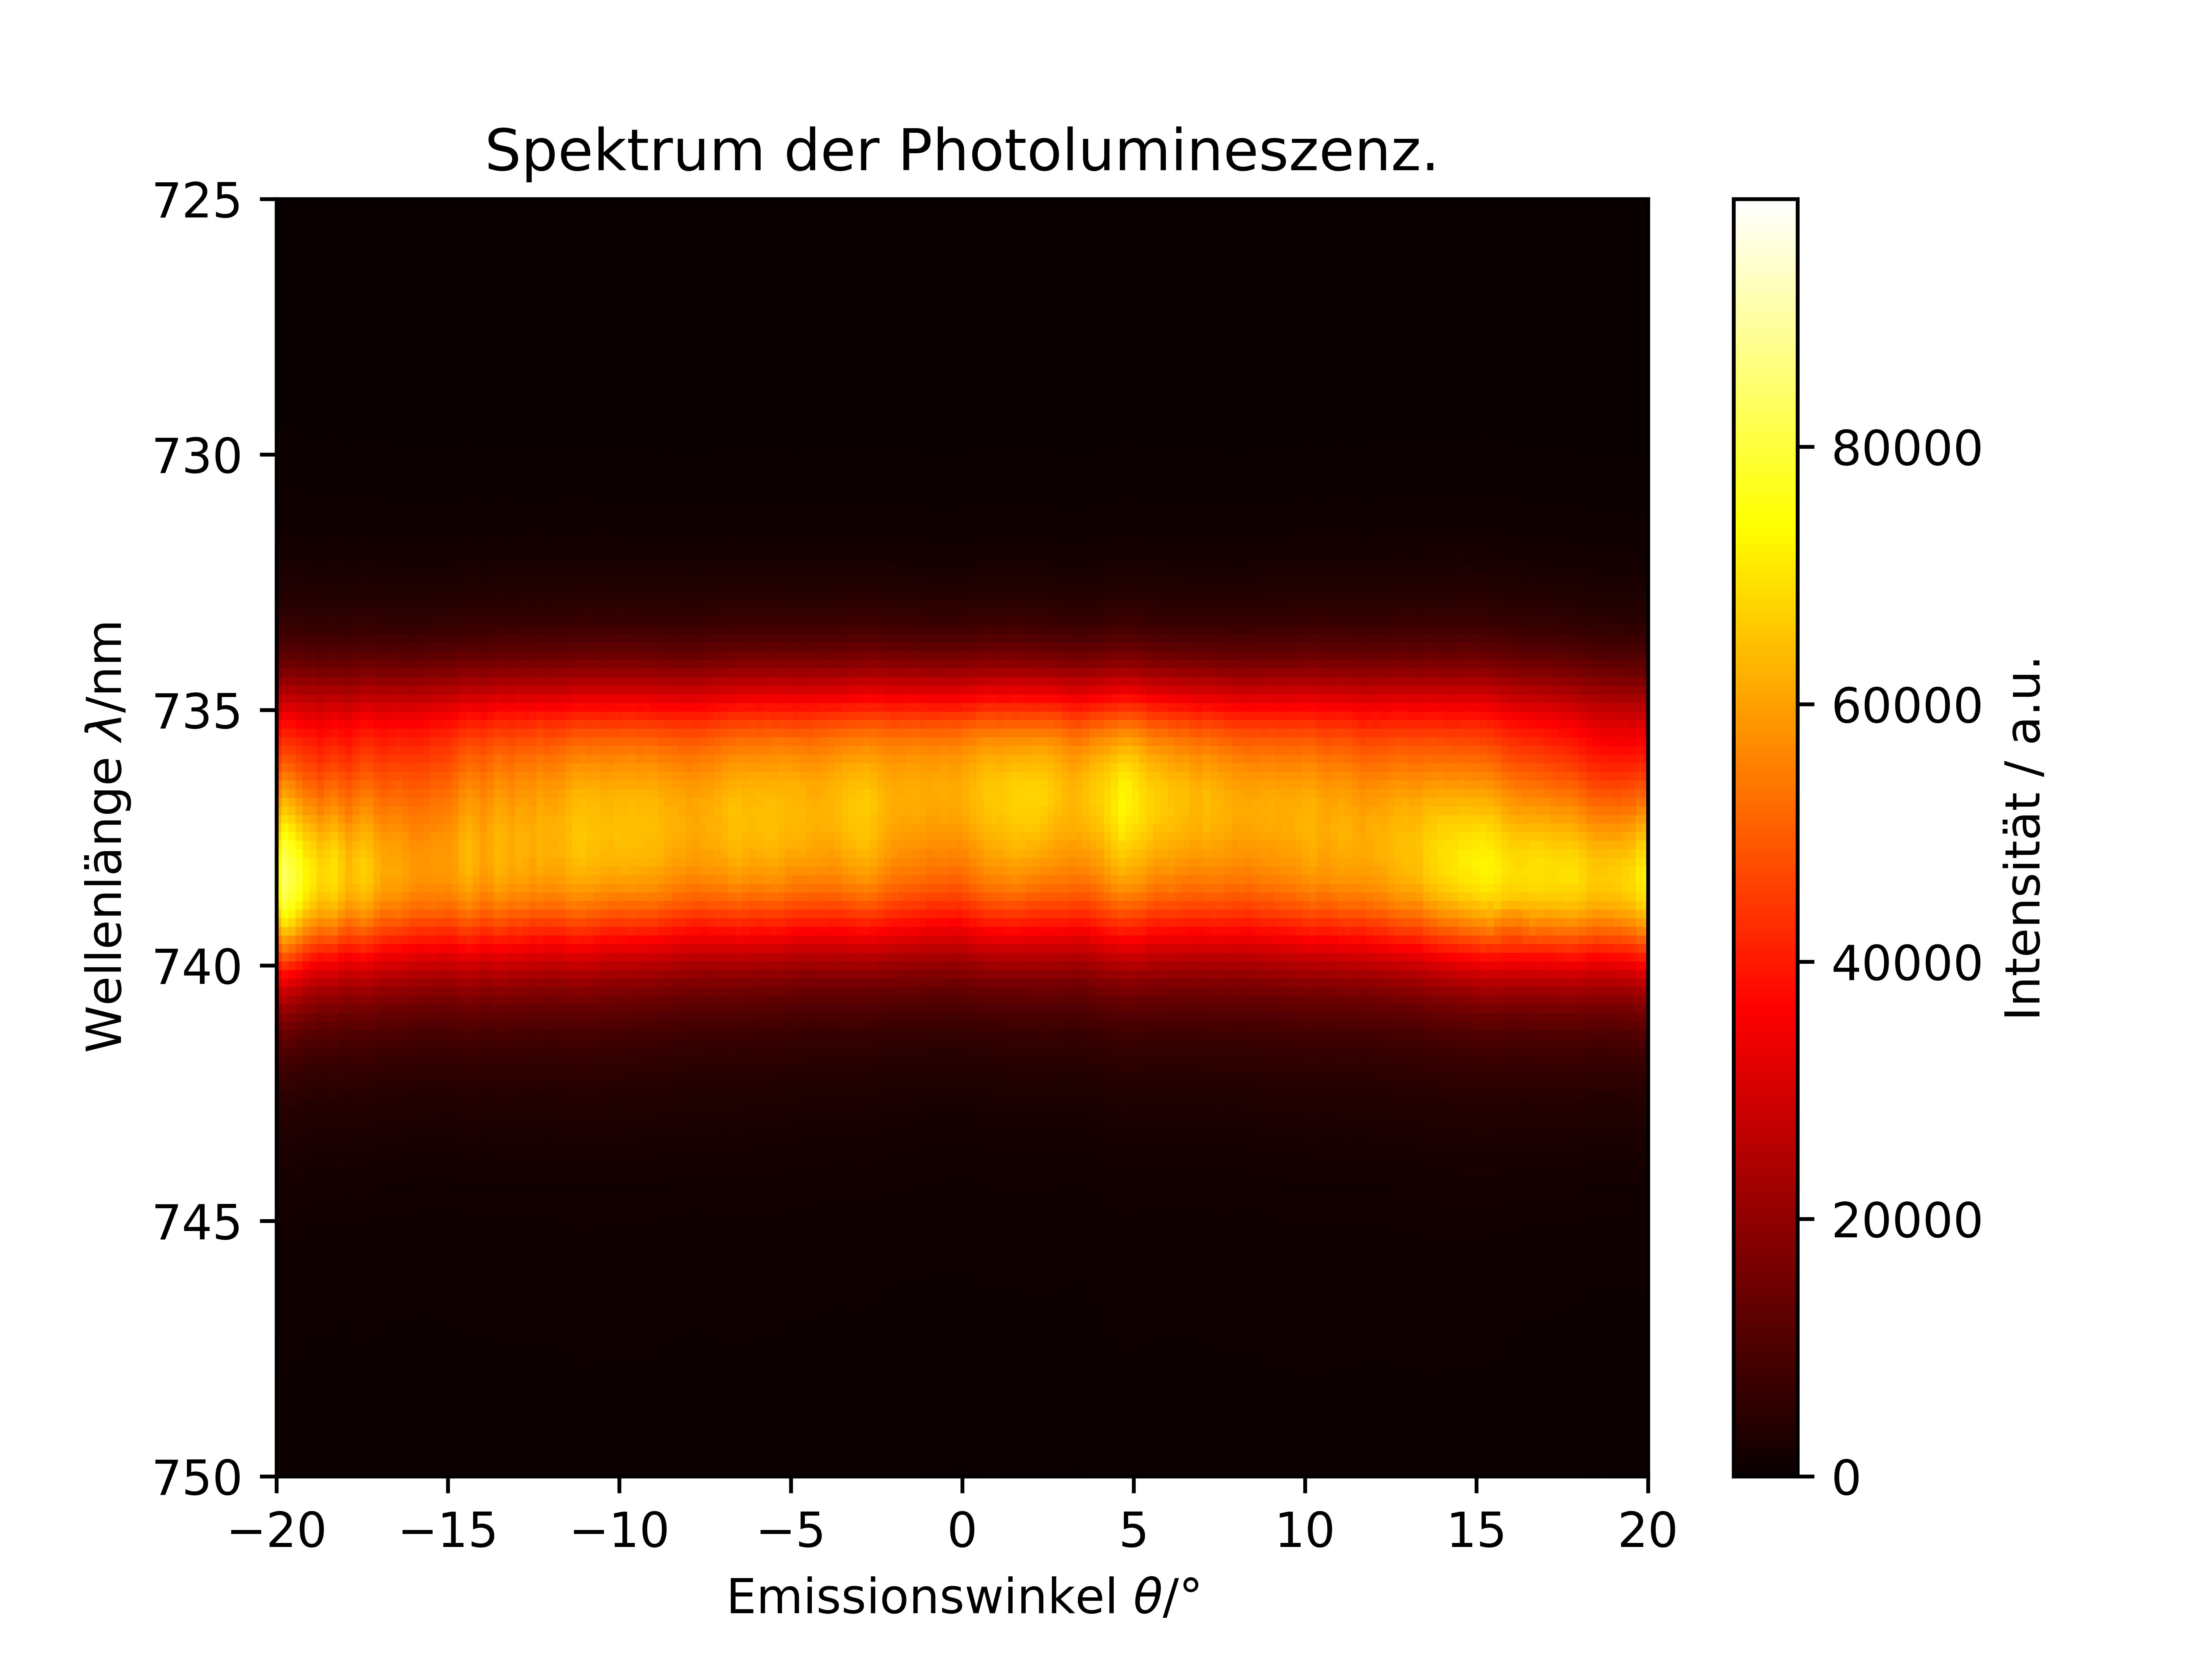
\includegraphics[scale=0.7]{./Plots/colormap__intensity_photolumineszenz_022818A 250nm 4K 2020-07-14.png}
    \caption{Darstellung des Intensitätsspektrum der Photolumineszenz.
    Die Temperatur  am Temperatursensor beträgt zum Zeitpunkt der Messung $\SI{4}{\kelvin}$. 
    Das Maximus der PL ist bei $\SI{737}{\nano\meter}$ mit einer Halbwertsbreite von ca. $\SI{5}{\nano\meter}$. 
    Je heller die Bereiche desto mehr Intensität ist an der Stelle gemessen worden.}
    \label{fig:photo}
\end{figure}
\FloatBarrier

In Abbildung~\ref{fig:i_pn} sind die unterschiedlichen Intensitätsverläufe bei positiven und negativen
Magnetfeld im Maximum der PL und in Abhängigkeit des Emissionswinkels zu sehen.
Für die Erstellung des Graphen wurde bei der Wellenlänge $\lambda = \SI{737}{\nano\meter}$ 
über insgesamt 40 Pixel der CCD gemittelt.
Das entspricht bei Umrechnung in eine Wellenlängenänderung einen Wert von $\pm \SI{7}{\nano\meter}$.

Bei Betrachtung positiver Winkel lässt sich erkennen, das dort die Probe mehr Licht bei negativen
Magnetfeld emittiert als bei positiven.
Eine Umkehrung des Intensitätsverlaufs ist bei Betrachtung negativer Winkel zu sehen.
Dieser Umstand deckt sich mit der vorrangestellten Theorie, da nun zirkular polarisierte Exzitonen mit dem 
umgekehrten Drehsinn entstehen und an Plasmonen mit entgegengesetzter Ausbreitungs- und Emissionsrichtung koppeln
(vgl. Abbildung~\ref{fig:zeeman}, $\sigma^- \leftrightarrow \sigma^+$).
Bei genauerer Betrachtung fällt auf, dass die beiden Graphen sich leicht links neben der $\SI{0}{\degree}$
Markierung schneiden.
Demnach muss es bei der durchgeführten Messung ($T = \SI{4}{\kelvin}$) zu äußeren Störungen gekommen sein.
\begin{figure}
    %\centering
    \begin{subfigure}{0.5\textwidth}
       %\centering
        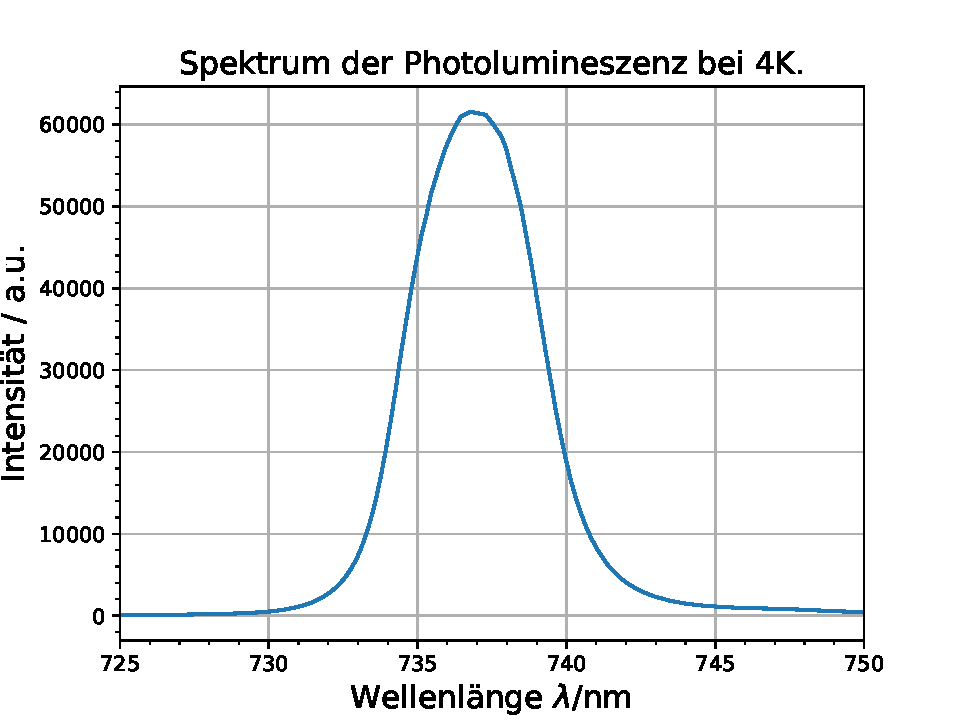
\includegraphics[scale=0.45]{./Plots/max_value_Pl_single.pdf}
        \caption{}
        \label{fig:max}
    \end{subfigure}
    \begin{subfigure}{0.5\textwidth}
        %\centering
        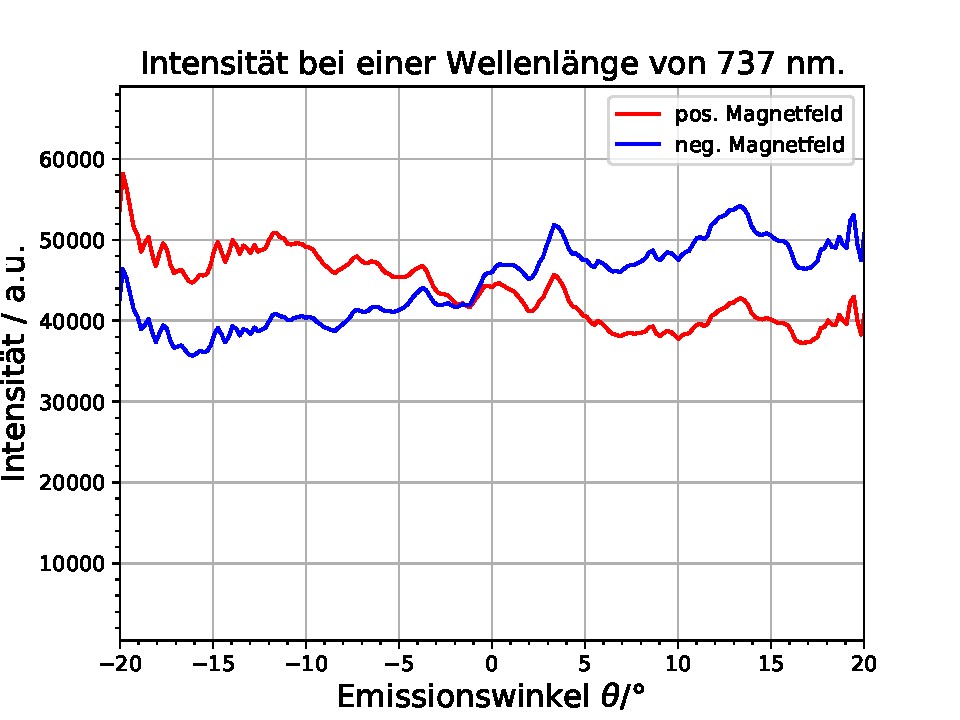
\includegraphics[scale=0.45]{./Plots/positive_and_negative_intensity_at_specific_wavelength_737_nm_022818A 250nm 4K 2020-07-14.pdf}
        \caption{}
        \label{fig:i_pn}
    \end{subfigure}
    \caption{(a) Darstellung des Intensitätsmaximums, der im Experiment gemessenen Photolumineszenz,
             der Probe in Abhängigkeit der Wellenlänge und bei $\SI{4}{\kelvin}$.
             (b) Darstellung des Intensitätsverlaufs der Probe beim Wechsel von positiven zu negativen Magnetfeld.
             Der Graph ist im Winkelbereich von $\SI{-20}{\degree}$ bis $\SI{20}{\degree}$ dargestellt.
              }
    \label{fig:rho}
\end{figure}
\FloatBarrier
%%%%%%%%%%%%%%%%%%%%%%%%%%%%%%%%%%%%%%%%%%%%%%%%%%%%%%%%%%%%%%%%%%%%%%%%%%%%%%%%%%%%%%%%%%%%%%%%%%%
%\begin{figure}
%    \centering
%    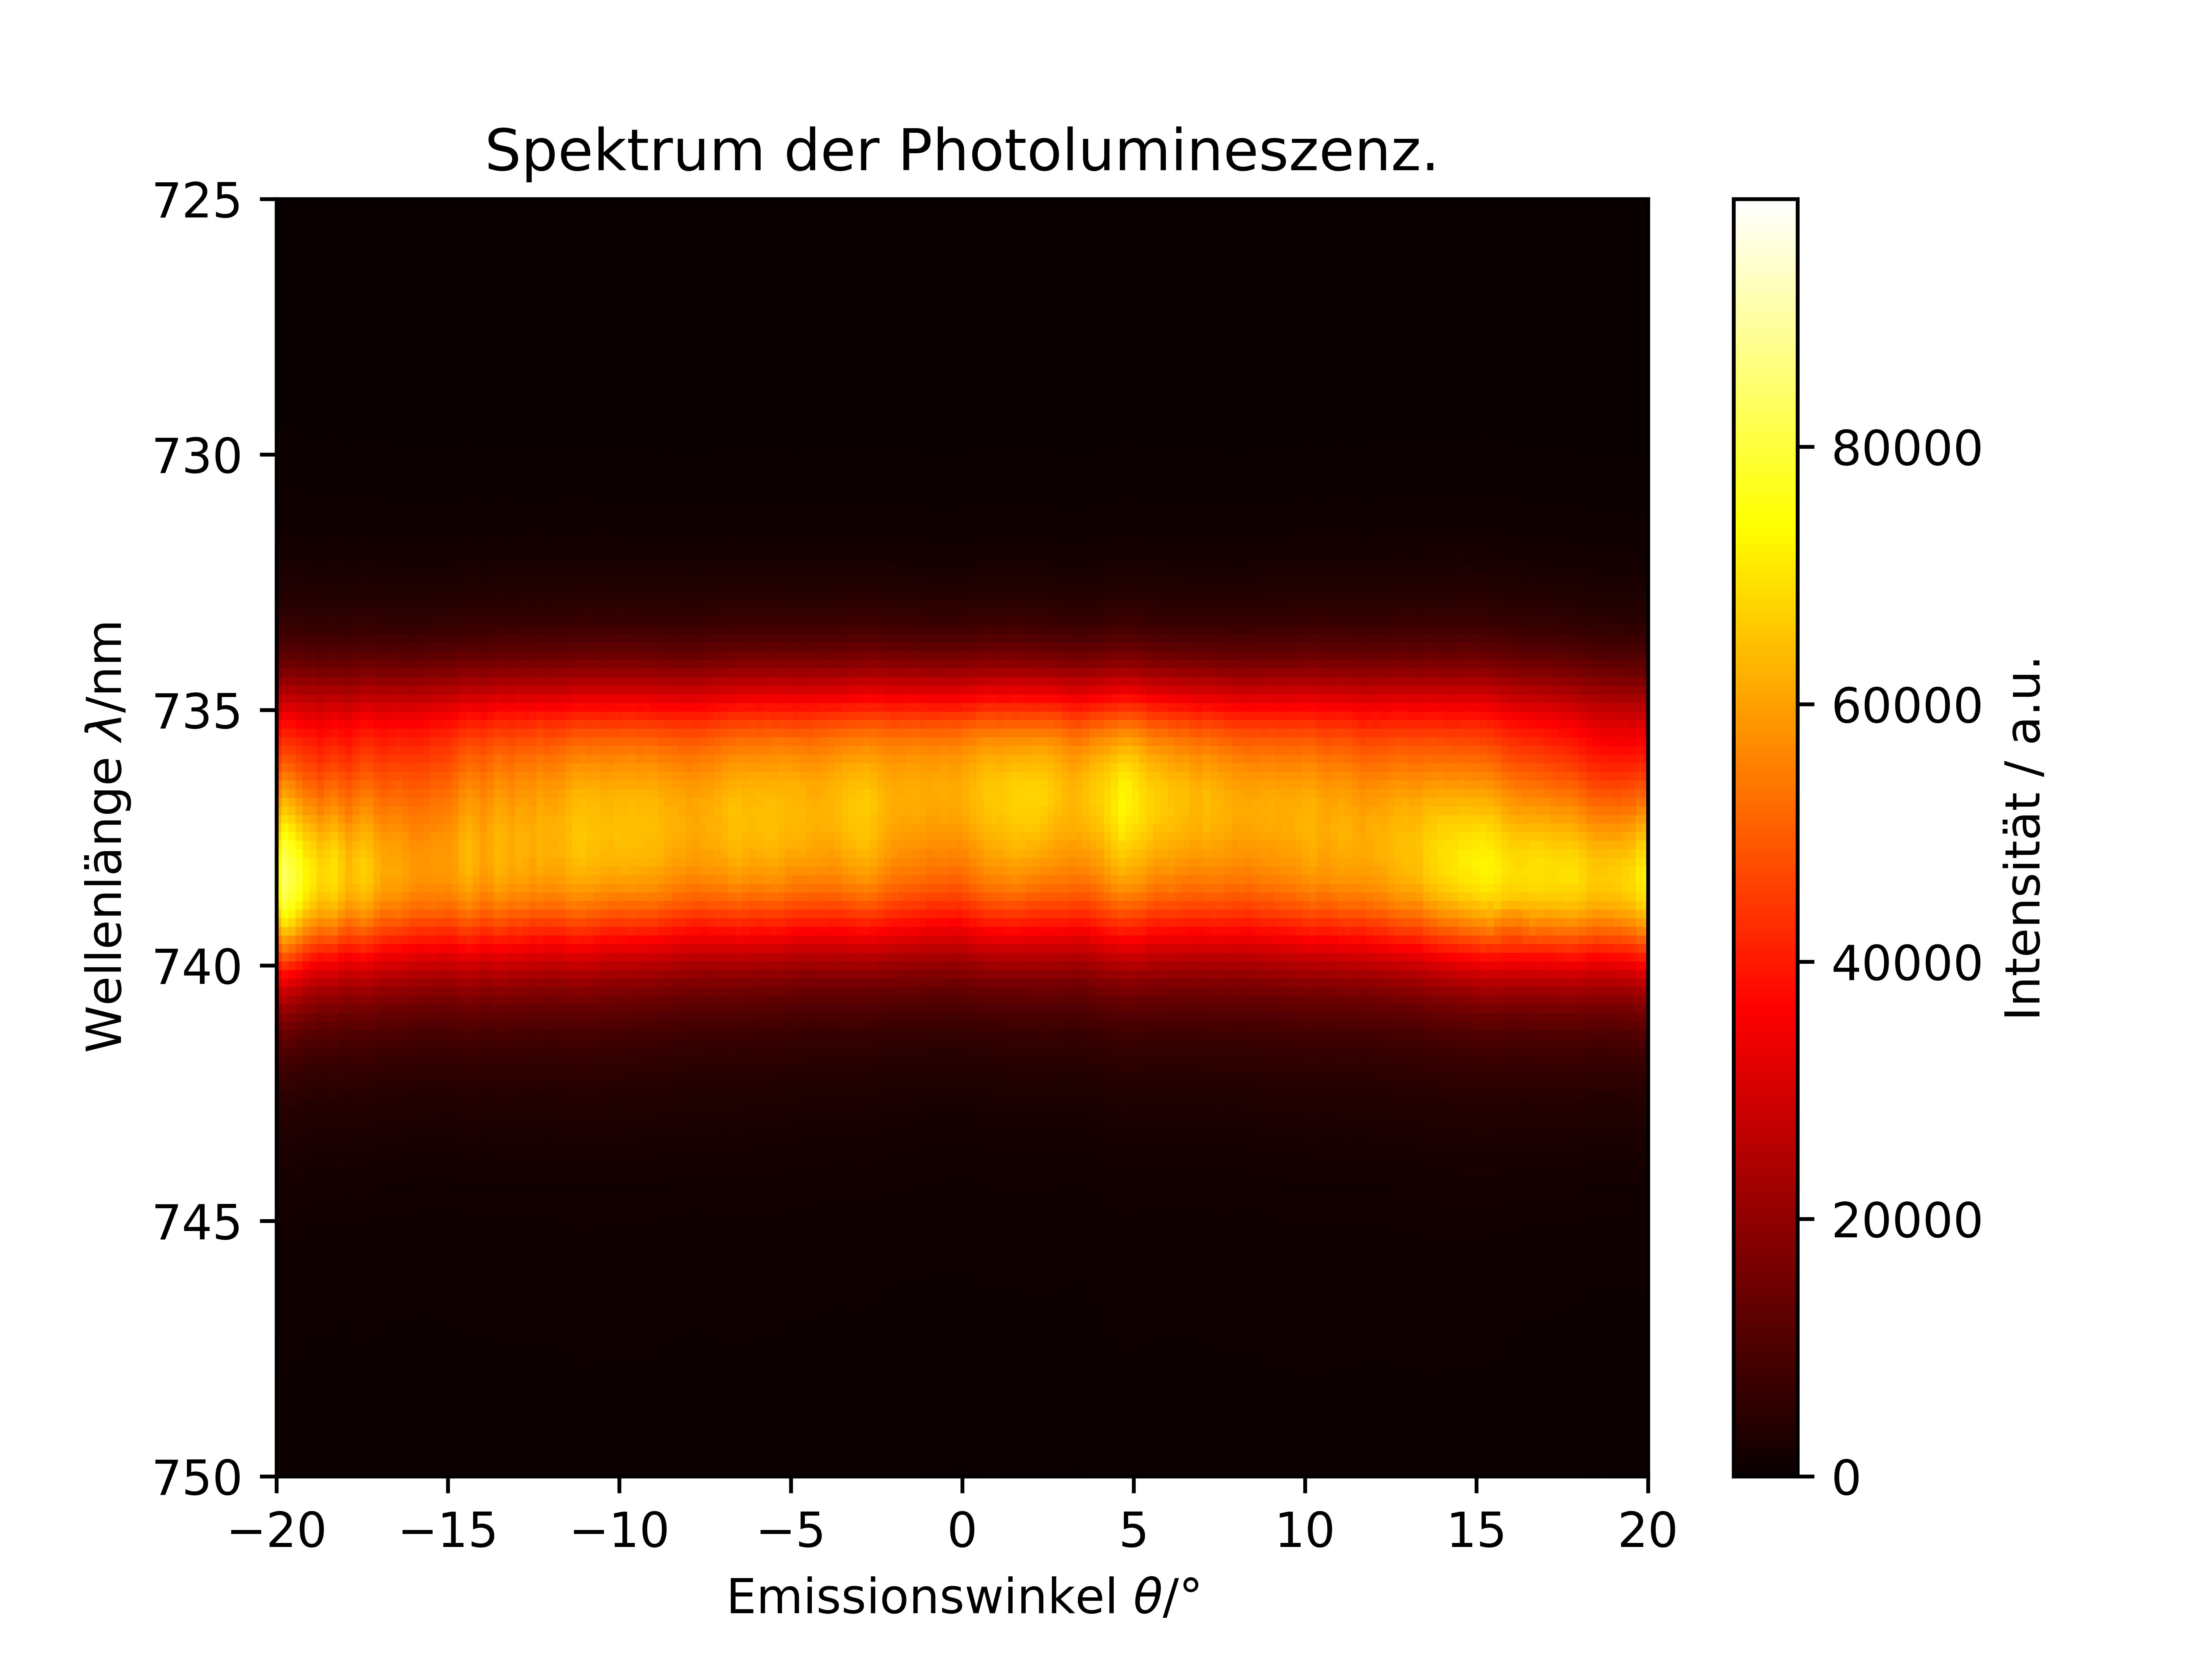
\includegraphics[scale=0.6]{./Plots/colormap__intensity_photolumineszenz_022818A 250nm 4K 2020-07-14.png}
%    \caption{Gemessene PL bei einer Temperatur von $\SI{4}{\kelvin}$. 
%    Das Maximus ist bei $\SI{737}{\nano\meter}$. 
%    Je heller die Bereiche desto mehr Intensität ist an der Stelle gemessen worden.}
%    \label{fig:photo}
%\end{figure}
%\FloatBarrier
Um die Änderung des Intensitätsverlaufs welcher in Abbildung~\ref{fig:i_pn} zu sehen ist zu quantifizieren
lässt sich die Größe $\rho$ definieren. 
Diese wird als relative Änderung der Intensität bezeichnet.
Die relative Änderung $\rho$ in Prozent gibt an, 
wie sehr sich die Lichtemission, für einen bestimmten Winkel und Wellenlänge, bei Umpolung des Magnetfelds ändert. 
Der Maximalwert von $\rho$ beträgt somit $1$.
Die neudefinierte Größe wird mit 
\begin{equation}
    \rho = \frac{I_\text{B+} - I_\text{B-} }{ I_\text{B+} + I_\text{B-} }
\end{equation}
berechnet.\\
Dabei ist $I_\text{B+}$ die Intensität bei positiven Magnetfeld und $I_\text{B-}$ bei negativen Magnetfeld.

Die im Experiment errechnete relative Änderung der Intensität,
über den vollständigen Wellenlängenbereich und in Abhängigkeitdes Emissionswinkels,
ist farblich in Abbildung~\ref{fig:rel_komplett} zu sehen.
Ein Teilausschnitt  ist in Abbildung~\ref{fig:rel} dargestellt.
Für beide Graphen wird ein Winkelbereich von $\pm \SI{20}{\degree}$ verwendet.
\begin{figure}
    %\centering
    \begin{subfigure}{0.50\textwidth}
        %\centering
        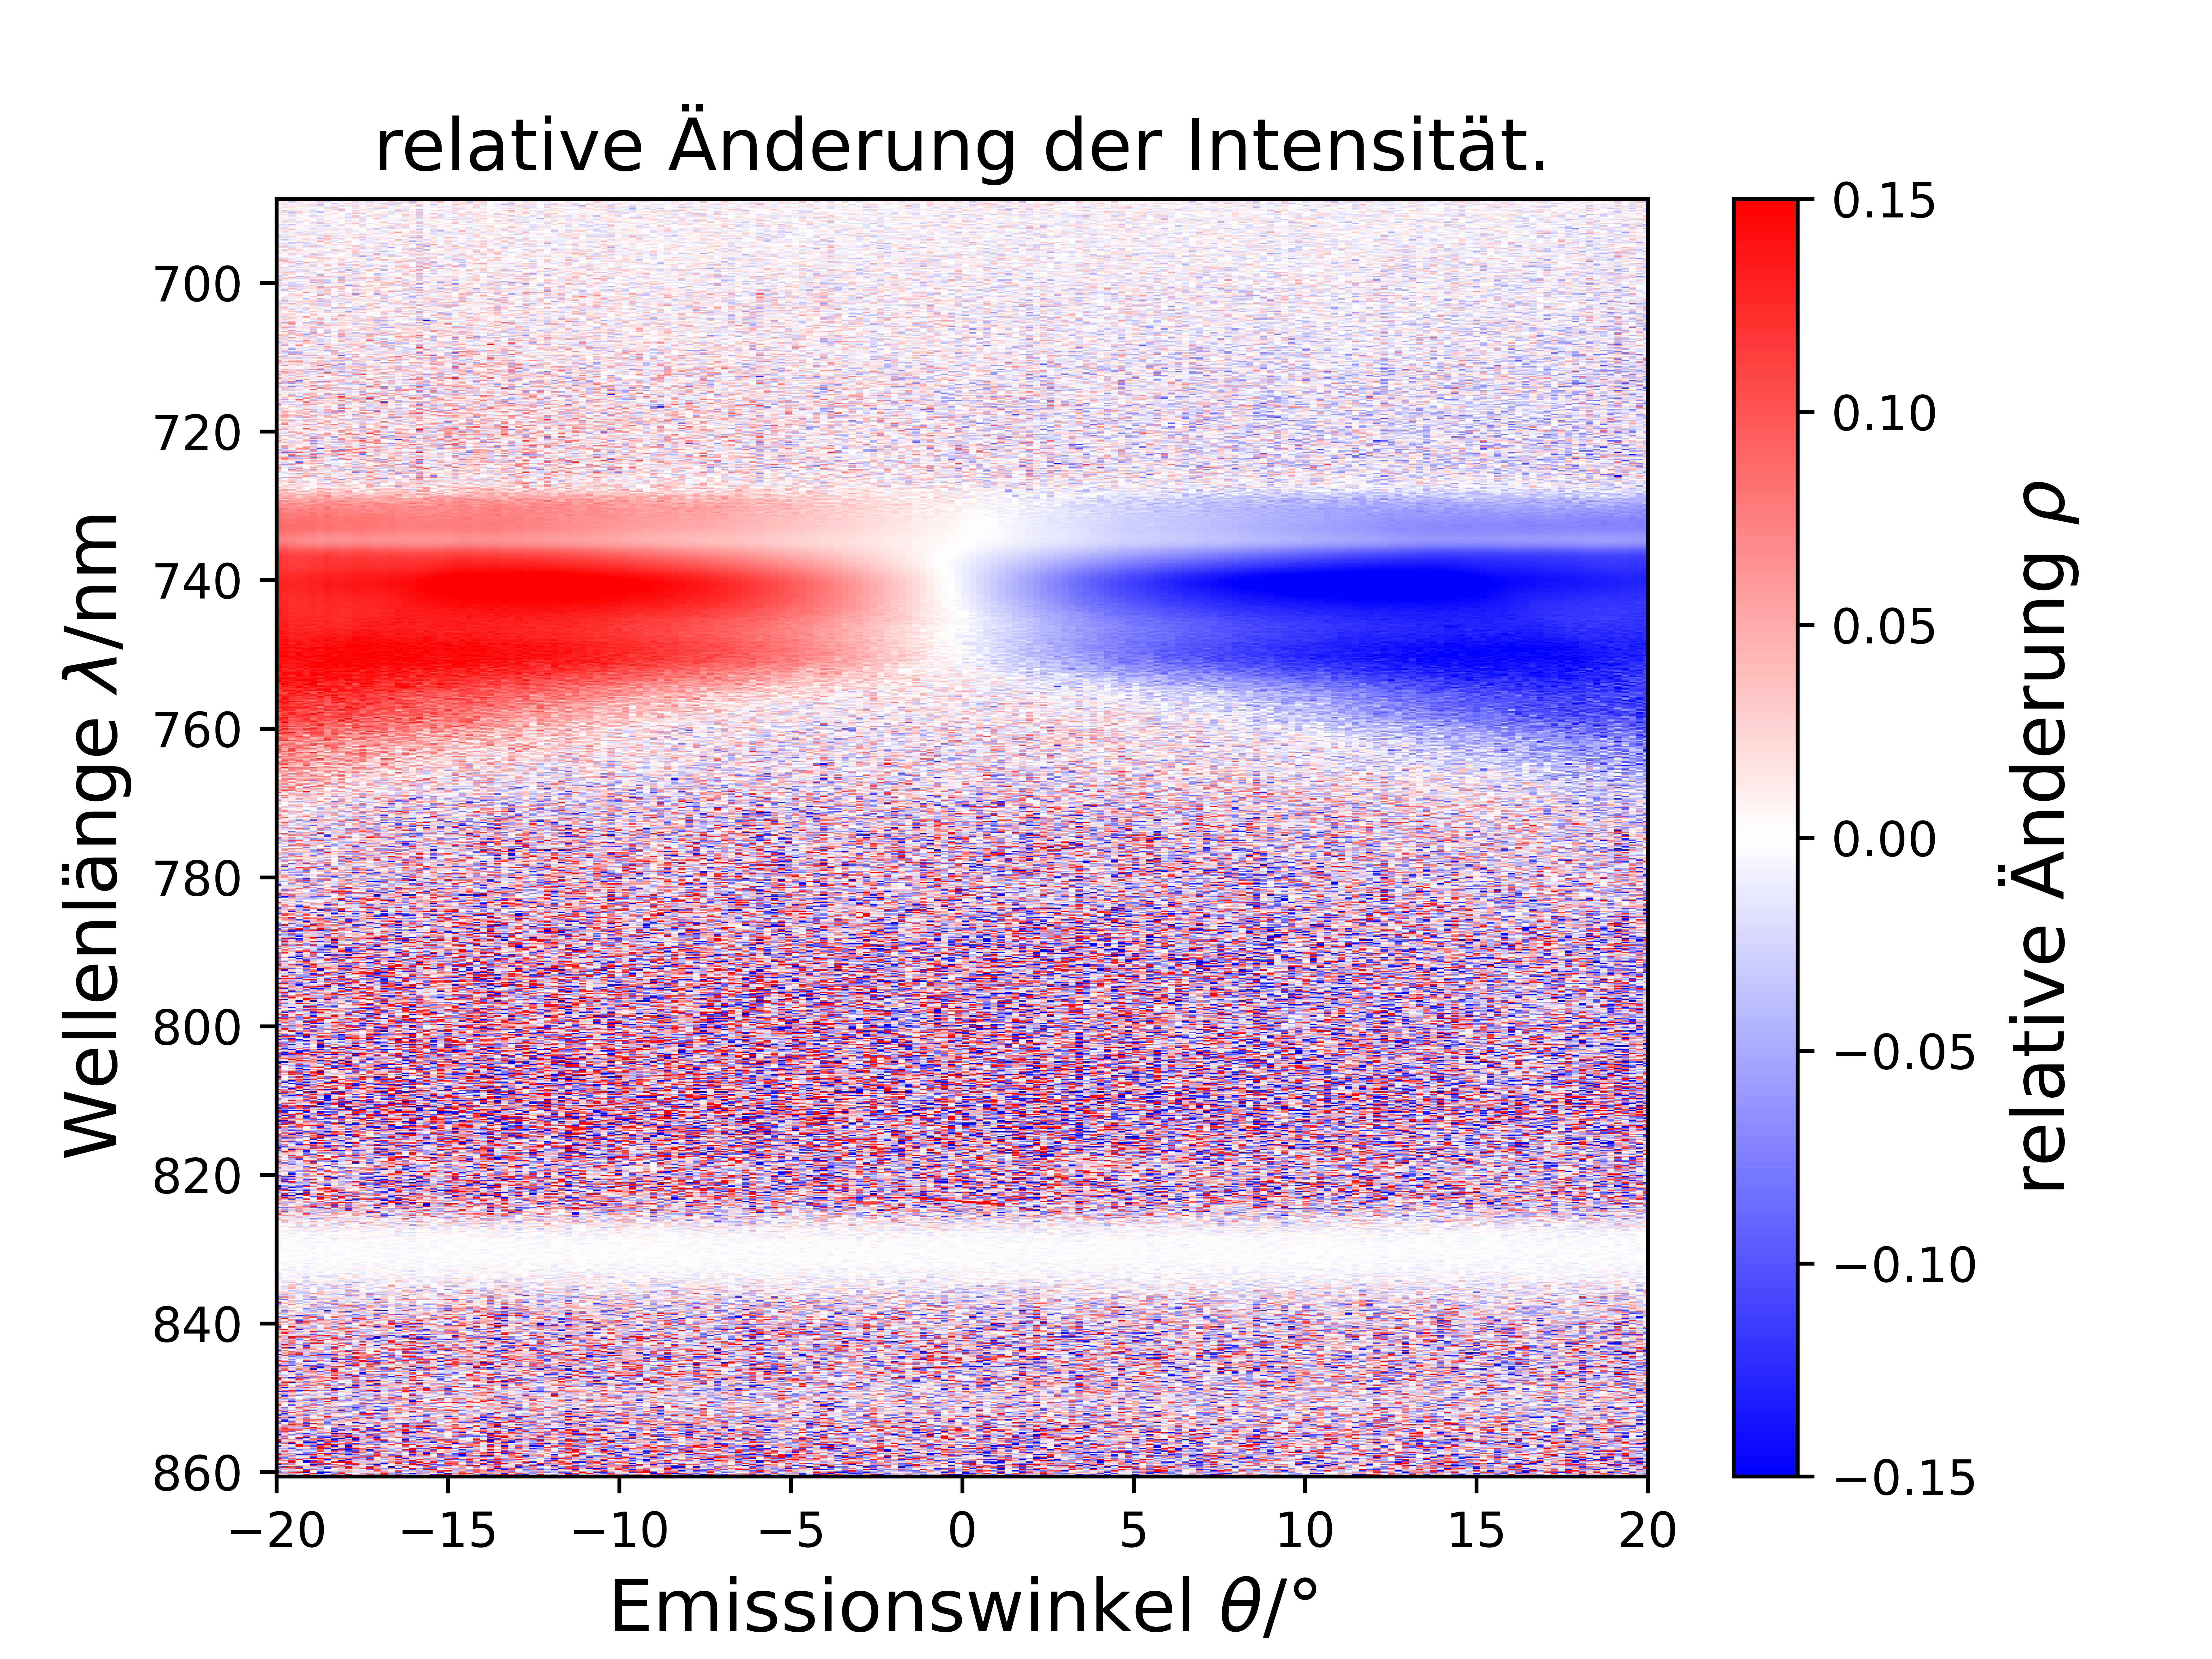
\includegraphics[scale=0.45]{./Plots/colormap_rel_change_intensity_022818A 250nm 4K 2020-07-14_komplett.png}
        \caption{}
        \label{fig:rel_komplett}
    \end{subfigure}
    \begin{subfigure}{0.50\textwidth}
        %\centering
        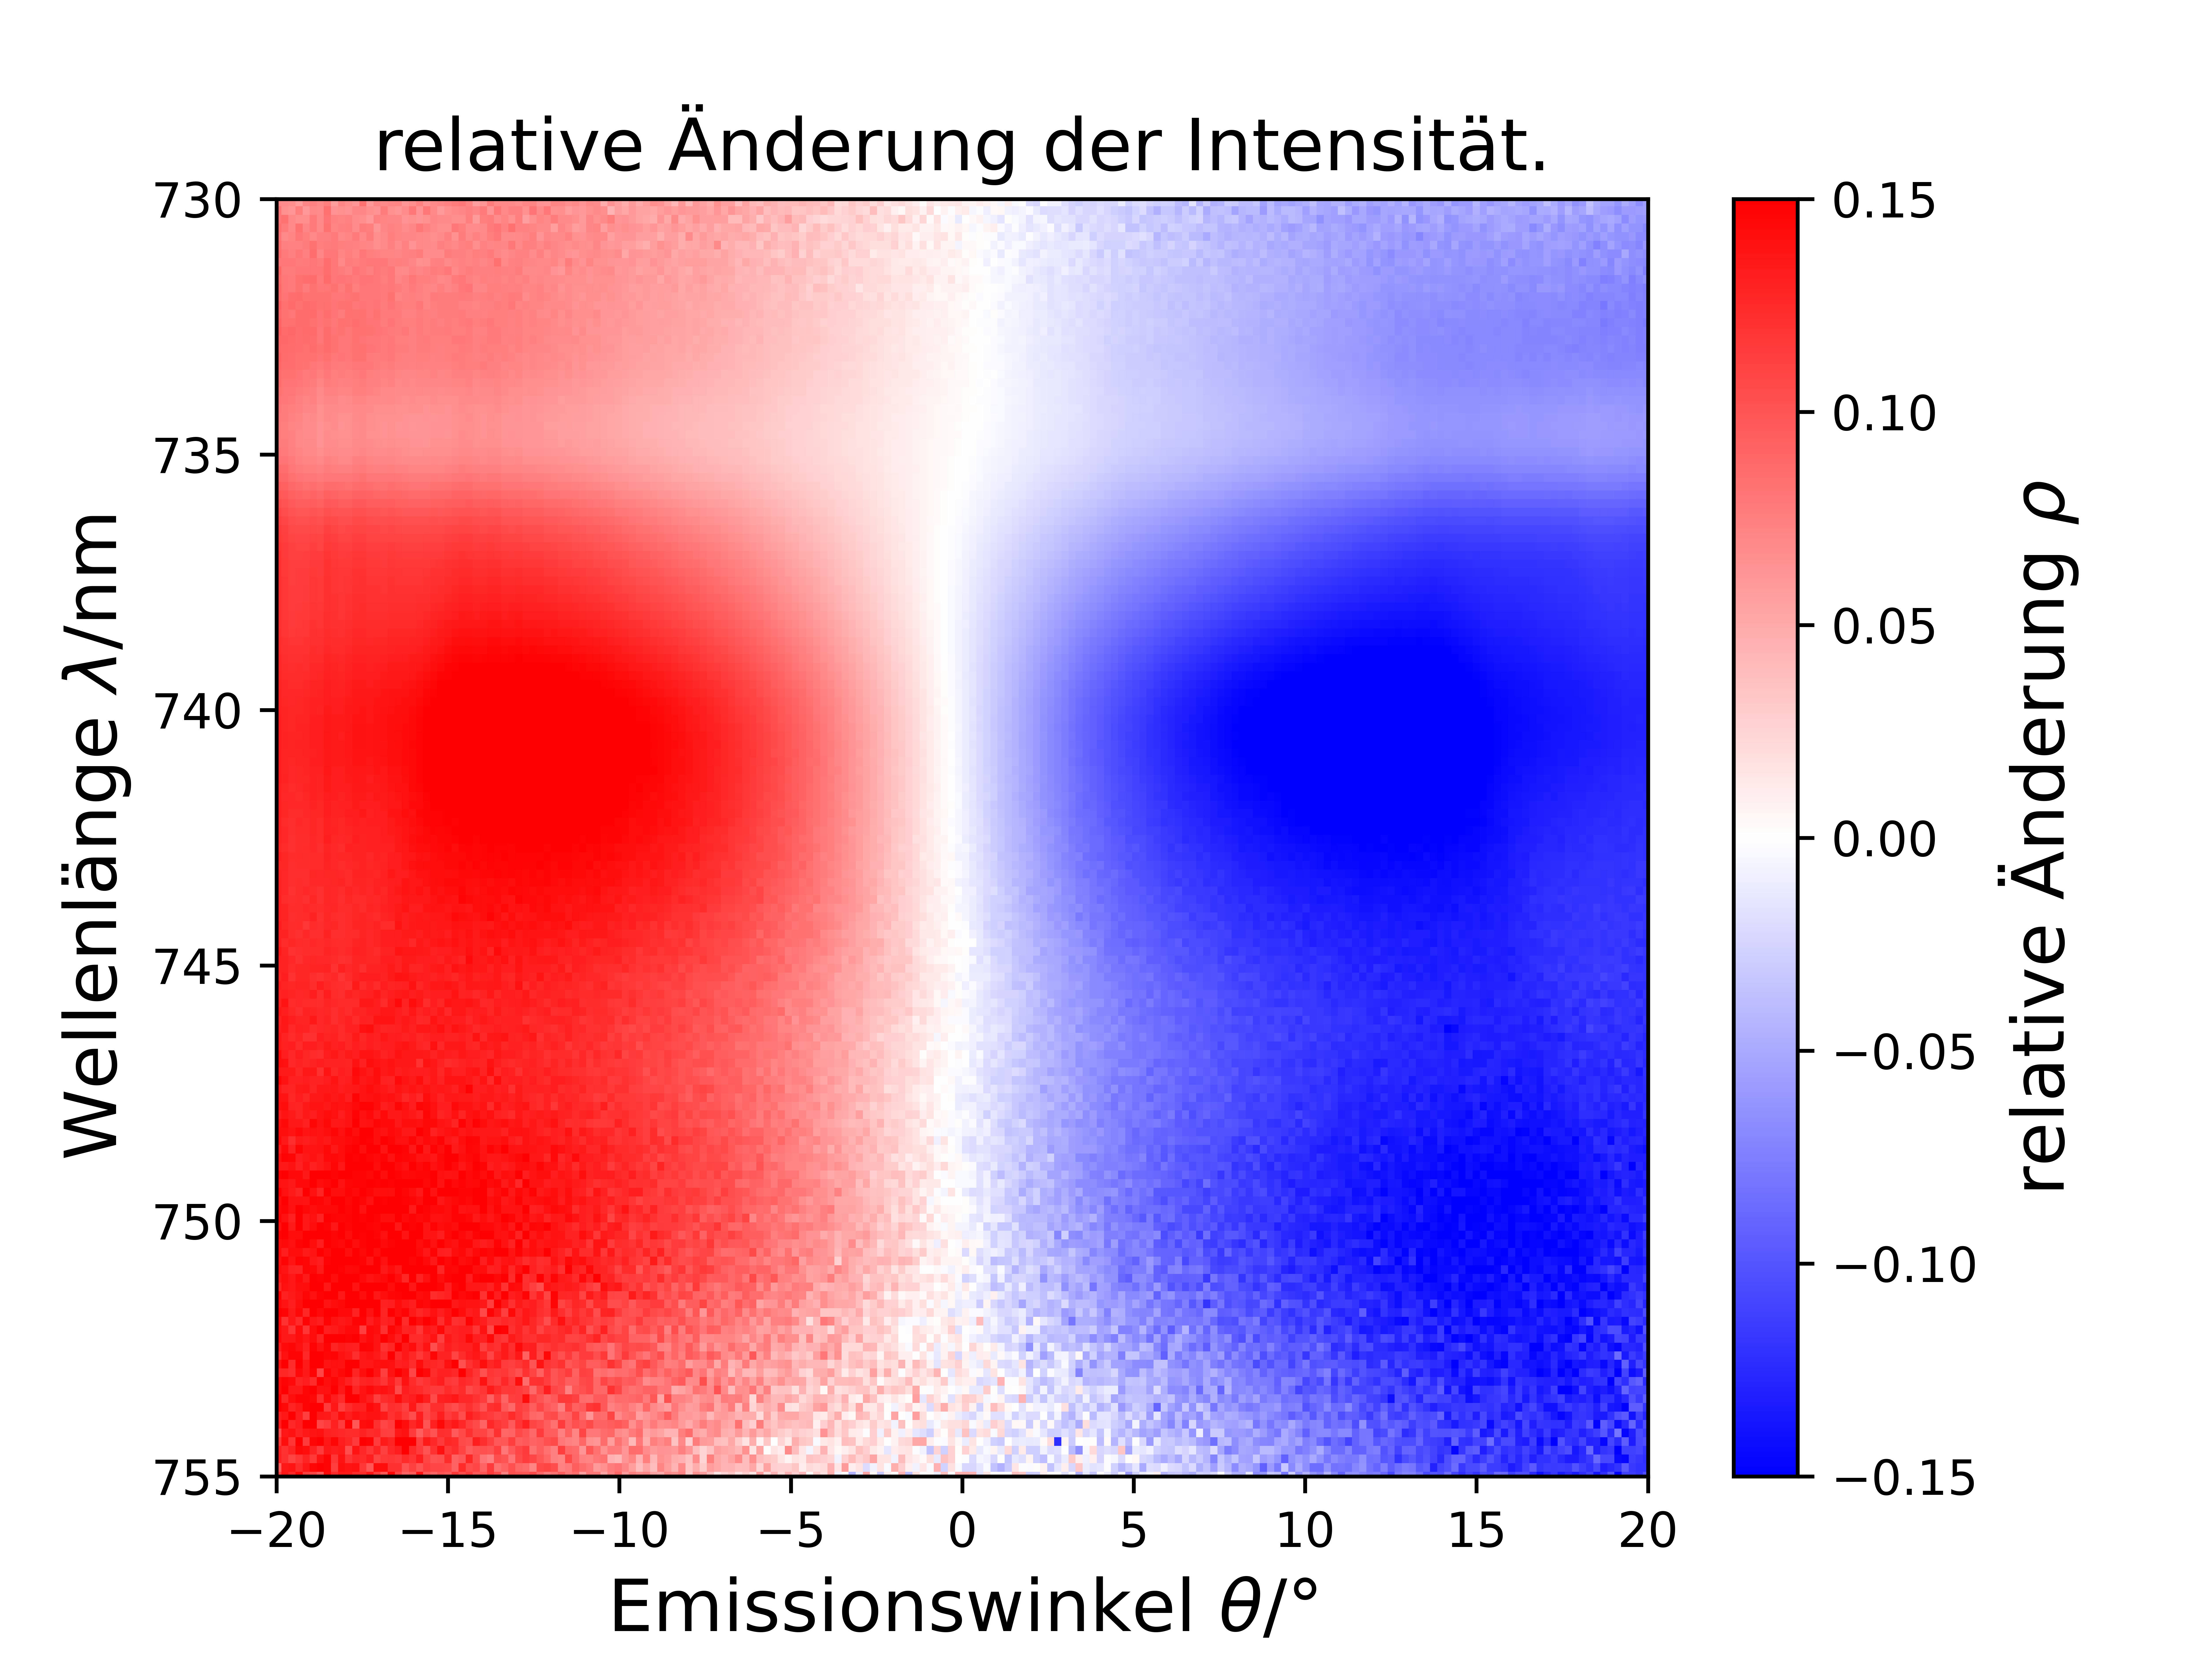
\includegraphics[scale=0.45]{./Plots/colormap_rel_change_intensity_022818A 250nm 4K 2020-07-14.png}
        \caption{}
        \label{fig:rel}
    \end{subfigure}
    \caption{(a) Gemessene relative Änderung der Intensität, über den kompletten Wellenlängenbereich, 
    bei einer Temperatur von $\SI{4}{\kelvin}$.(b) Gemessene relative Änderung der Intensität im Bereich
     von $\SI{730}{\nano\meter}$ bis $\SI{755}{\nano\meter}$
        bei einer Temperatur von $\SI{4}{\kelvin}$.}
    \label{fig:rho}
\end{figure}
\FloatBarrier
Der maximal gemessene Wert von $\rho$ im Experiment beträgt $\pm \SI{15}{\percent}$. 
Wird Abbildung~\ref{fig:rel_komplett} genauer betrachtet fällt auf, dass sich die 
relative Änderung im wesentlichen auf den Bereich zwischen $\SI{730}{\nano\meter}$ und $\SI{755}{\nano\meter}$
beschränkt.
Das ist im Graphen anhand der unterschiedlichen Farbintensitäten zu erkennen. 
In diesem Bereich ist für positive Emissionswinkel die relative Änderung $\rho$ negativ.
Für negative Winkel ist $\rho$ positiv.
Der weiße Balken der im Wellenlängenbereich von ca. $\SI{825}{\nano\meter}$ bis $\SI{835}{\nano\meter}$ 
in Abbildung\ref{fig:rel_komplett} zu sehen ist, 
hat seinen Ursprung im verwendten Substrat GaAs. 
Da dieses ebenfalls zum Leuchten angeregt wird.
GaAs hat allerdings keine magnetischen Eigenschaften, 
darum entfällt die Beeinflussung durch das angelegte Magnetfeld
und es ist keine relative Änderung erkennbar.
Somit erscheint diese Stelle im Graphen weiß.
Der Restbereich, d.h. der Bereich ohne Signifikanten Effekt, besteht aus einem statistischen Pixelrauschen der CCD.

In Abbildung~\ref{fig:rel} ist der Bereich um das Emissionsmaximum des Quantentopfes dargestellt.
Der Wellenlängenbereich liegt zwischen $\SI{730}{\nano\meter}$ und $\SI{755}{\nano\meter}$.
In der Mitte des Graphen bei $\theta = \SI{0}{\degree}$ ist eine weißer vertikaler Liniebereich zu erkennen.
Dieser Bereich entsteht da bei einem Winkel von $\theta = \SI{0}{\degree}$ das PL genau senkrecht aus der Probe kommt
und somit keine Direktionalität aufweisen kann.
Wird der Bereich um  $\lambda = \SI{735}{\nano\meter}$ betrachtet 
lässt sich eine schwächere Farbintensität erkennen.
Das bedeutet das dort die relative Änderung $\rho$  kleiner ist also sich das emittierte Licht 
weniger gut durch das angelegte Magnetfeld steuern lassen hat.
Vorhergehende Messungen haben ergeben, das das Maximum der PL ohne Goldgitter bei 
einer Wellenlänge von $\lambda = \SI{735}{\nano\meter}$ liegt.
Dadurch kommt wahrscheinlich eine Überlagerung Zustande und 
es wird vermutet, das dieses Licht aus den Randbereichen der Probe und/oder aus den Zwischenbereichen des Goldgitters 
emittiert wird.
Im Wellenlängenbereich zwischen $\SI{738}{\nano\meter}$ und $\SI{740}{\nano\meter}$ lässt durch die intensive
Farbintensität erkennen, das hier die beste Steuerung der Lichtemission, durch das Magnetfeld gelungen ist.

Wird die relative Änderung der Intensität $\rho$ in Abhängigkeit des Winkelbereichs und bei 
konstanter Wellenlänge von $\lambda = \SI{737}{\nano\meter}$
betrachtet, ergibt sich der Graph in Abbildung~\ref{fig:dir}.
Es fällt auf das 
der Graph von $\rho$, bis auf eine kleine Abweichung am Nullpunkt,
antisymmetrisch ist.
Dieser Befund deckt sich mit den theoretischen Betrachtungen 
und den experimentellen Befunden an einer ähnlichen Probe \cite{felix}.

Bei genauerer Analyse des Graphen der Direktionalität lässt sich erkennen, dass bis ca. $\theta = \pm \SI{5}{\degree}$
die Steigung von $\rho$ linear ist.
Wird dieser Wert über- bzw. unterschritten geht der Graph in eine Krümmung über, die bei $\theta = \pm \SI{13,5}{\degree}$
ihr Maximum besitzt. 
Der dazugehörige Maximalwert beträgt $\rho = \SI{11,5}{\percent}$. 
Hinter dem Maximum schwächt sich die Direktionalität ab.
\begin{figure}
    \centering
    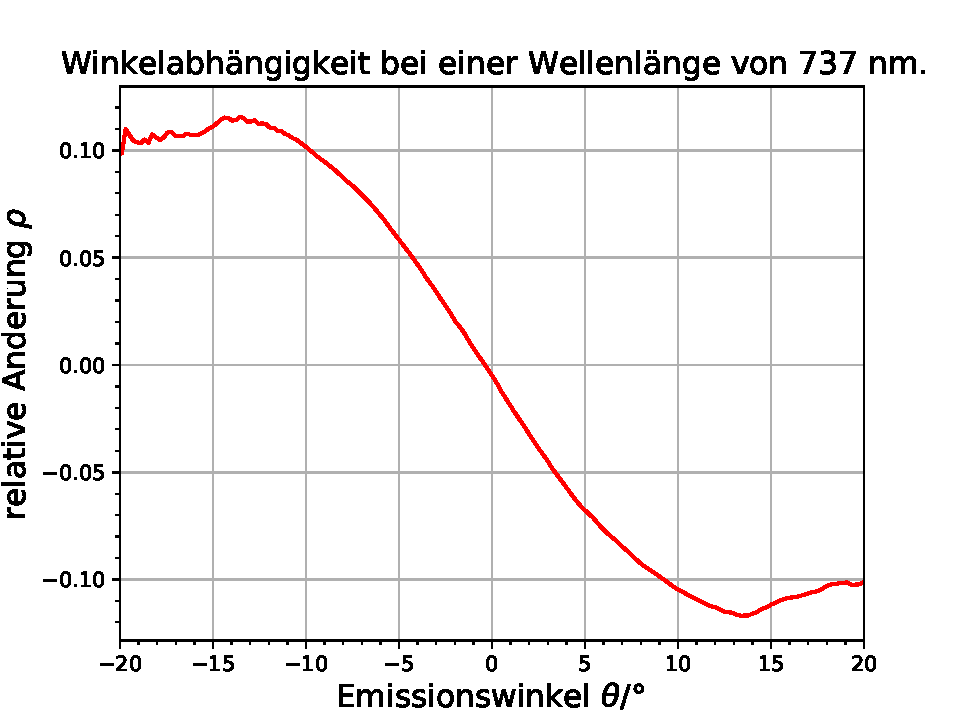
\includegraphics[scale=0.7]{./Plots/rho_at_specific_wavelength_737_nm_022818A 250nm 4K 2020-07-14.pdf}
    \caption{Gemessene Direktionalität $\rho$ im Maximum der Photolumineszenz.
    Der Wert der im Experiment gemessen Direktionalität ist $\rho = \SI{11,5}{\percent}$.}
    \label{fig:dir}
\end{figure}
\FloatBarrier
Da bereits in mehreren Experimenten unabhängig dieser von Arbeit bestätigt wird, dass der Graph
der Direktionalität antisymmetrisch ist, wird nur der antisymmetrische Anteil von $\rho$ betrachtet.  
Dazu wird der Direktionalitätsfaktor $C$, kurz Direktionalität, eingeführt. 

Es gilt 
\begin{equation}
    C= \frac{\rho(-\theta)-\rho(\theta)}{2}.
    \label{eq:C} 
\end{equation}

Durch die Direktionalität wird als nur der antisymmetrische Anteil von $\rho$ betracht.
Der Verlauf der Direktionalität ist in Abbildung~\ref{fig:dir_kor} zu sehen.
\begin{figure}
    \centering
    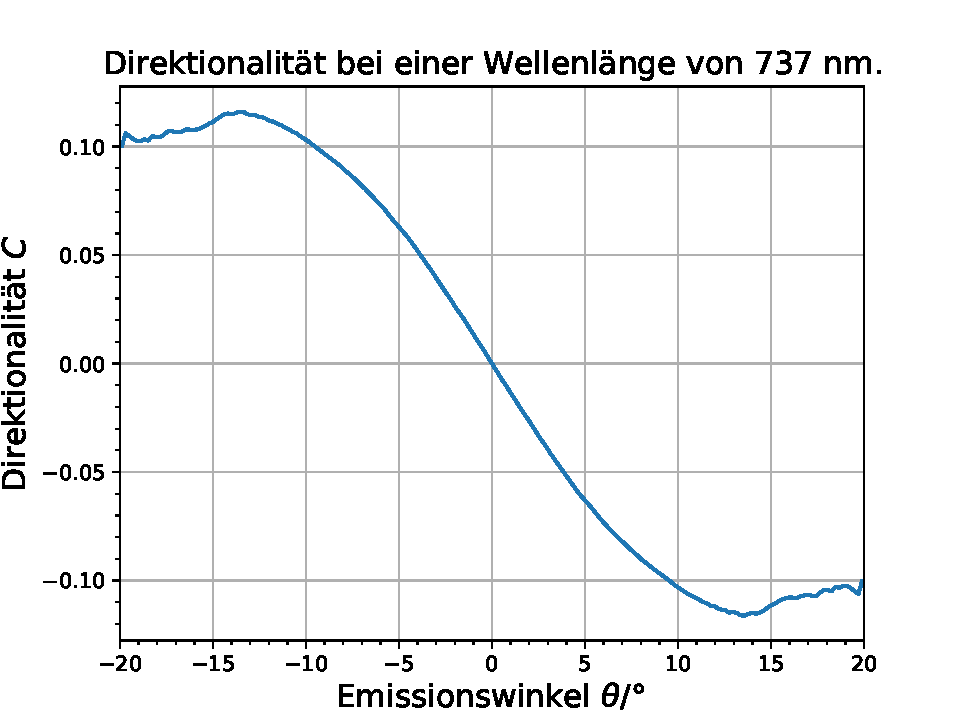
\includegraphics[scale=0.7]{./Plots/rho_at_specific_wavelength_737_nm_022818A 250nm 4K 2020-07-14_korrigiert.pdf}
    \caption{Darstellung des Verlaufs der Direktionalität $C$.
     Die Direktionalität $C$ unterscheidet sich von $\rho$ indem sie nur die antisymmetrischen
     Anteile berücksichtigt. Der Graph von $\rho$ unterscheidet sich nur geringfügig von dem hier 
     abgebildeten Verlauf, dies spricht für eine gewisse Genauigkeit der Messungen im Experiment. }
    \label{fig:dir_kor}
\end{figure}
\FloatBarrier


\section{Temperatur Abhängigkeit der Direktionalität}
Im folgenden Abschnitt der Arbeit wird die Temperaturabhängigkeit der im Experiment
beobachteten Direktionalität $C$ diskutiert und wesentliche Aspekte erläutert.

Die Probe wurde über einem Temperaturbereich von $ \Delta T =\SI{41}{\kelvin} $ gemessen.
Die kleinste eingestellte Temperatur ist dabei $T =\SI{4}{\kelvin}$ gewesen, die größte 
$T =\SI{45}{\kelvin}$.
Es sind insgesamt 11 temperaturabhängige Messungen entstanden.

Die Wellenlänge bei der alle nachfolgenden Graphen betrachtet werden ist $\lambda =\SI{738}{\nano\meter}$,
da sich das über alle Temperaturen gemittelte Maximum der Photolumineszenz bei
$\lambda =\SI{737,7}{\nano\meter}$ befindet.
Im Abbildung~\ref{fig:int_temp} sind die Intensitätsmaxima bei den unterschiedlichen Temperaturen zu sehen.
\begin{figure}
    \centering
    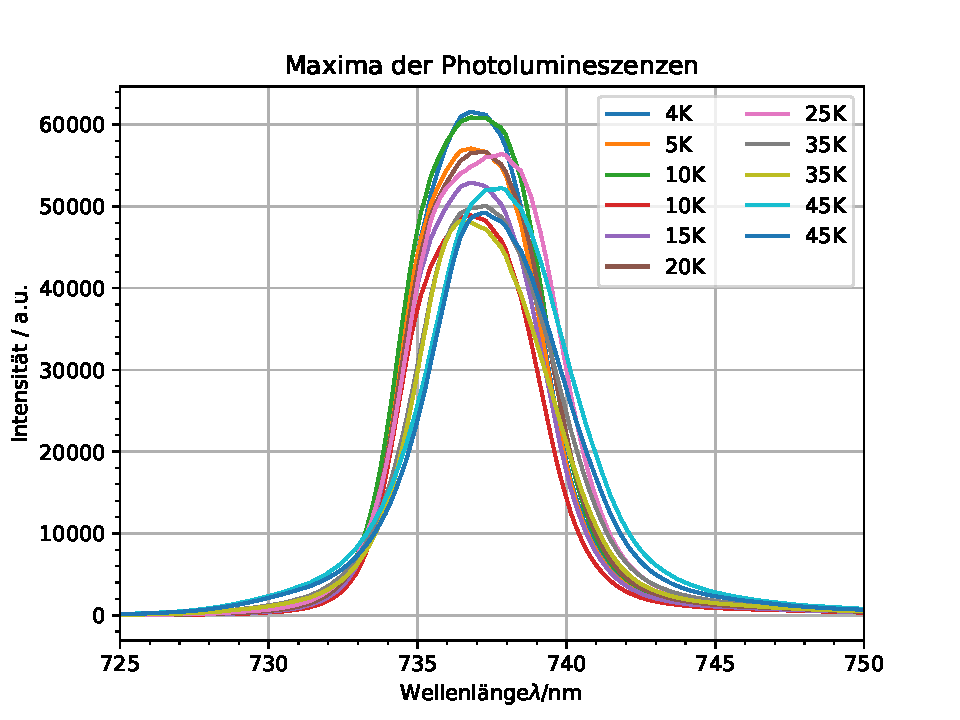
\includegraphics[scale=0.7]{./Plots/max_value_Pl_alle.pdf}
    \caption{Darstellung der Intensitätsmaxima bei unterschiedlichen Temperaturen.
    Das gemittelte Maxima ist bei $\lambda =\SI{737,7}{\nano\meter}$.}
    \label{fig:int_temp}
\end{figure}
\FloatBarrier 

In Abbildung~\ref{fig:temp_all_nach} sind winkelabhängigen Direktionalitäten, für die untersuchten Temperaturen,
bei konstanter Wellenlänge, abgebildet.
%\begin{figure}
%    \centering
%    \begin{subfigure}{0.55\textwidth}
%       %\centering
%        \includegraphics[scale=0.45]{./Plots/Temperaturabhaengigkeit_rho_at_738_nm_4K5K10K10K15K20K25K35K35K45K45K_vorher.pdf}
%        \caption{Darstellung der Direktionalität $\rho$ bei konstanter Wellenlänge und  unterschiedlichen Temperaturen.
%         Die Wellenlänge beträgt $\lambda =\SI{738}{\nano\meter}$.}
%        \label{fig:temp_all_vor}
%    \end{subfigure}
%    \begin{subfigure}{0.55\textwidth}
%        %\centering
%        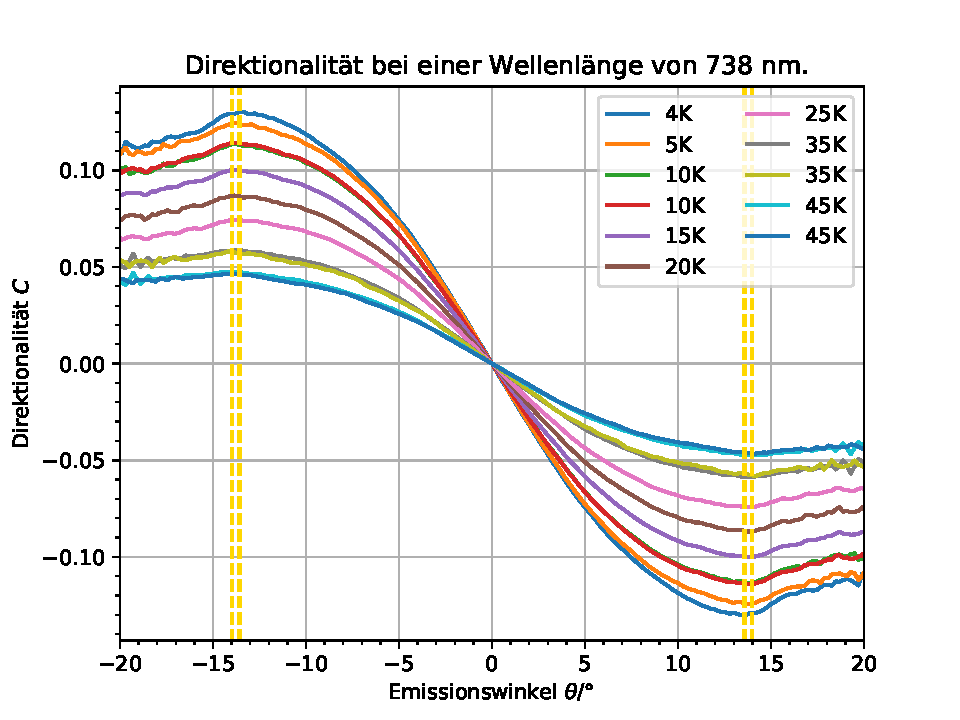
\includegraphics[scale=0.45]{./Plots/Temperaturabhaengigkeit_rho_at_738_nm_4K5K10K10K15K20K25K35K35K45K45K_korrigiert.pdf}
%        \caption{Darstellung der Direktionalität $C$ bei konstanter Wellenlänge und  unterschiedlichen Temperaturen.
%         Die Wellenlänge beträgt $\lambda =\SI{738}{\nano\meter}$.}
%        \label{fig:temp_all_nach}
%    \end{subfigure}
%    \caption{In der linken Abbildung ist die Direktionalität $\rho$ zu sehen, in der rechten der Direktionalitätsfaktor $C$.}
%    \label{fig:temp_verlauf}
%\end{figure}
%\FloatBarrier
%TODO fix der zeichnungen
\begin{figure}
    \centering
    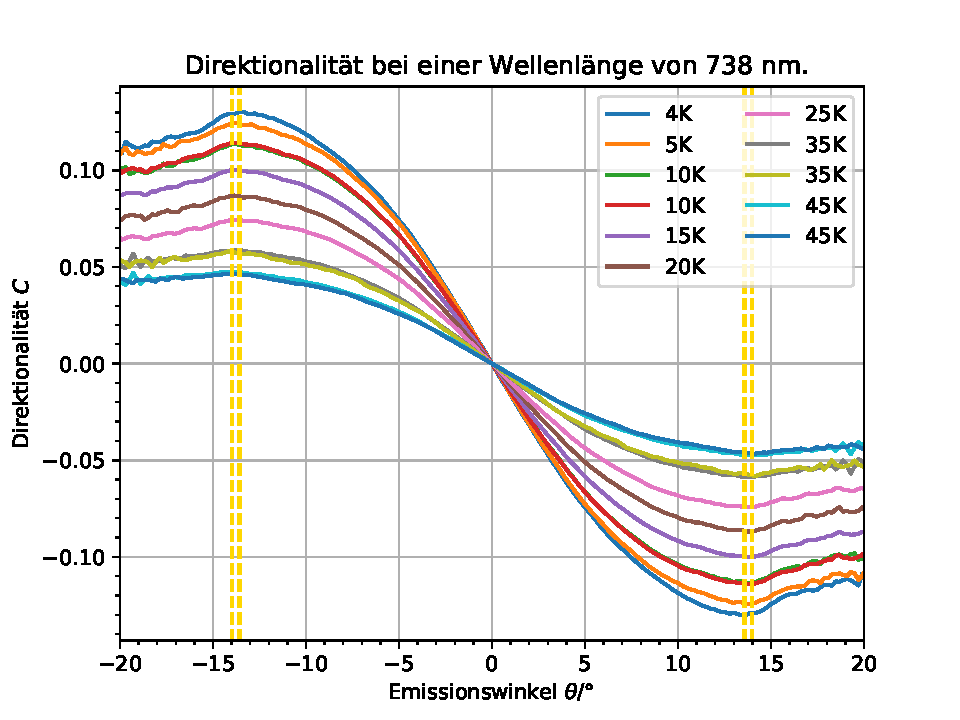
\includegraphics[scale=0.7]{./Plots/Temperaturabhaengigkeit_rho_at_738_nm_4K5K10K10K15K20K25K35K35K45K45K_korrigiert.pdf}
    \caption{Darstellung des Direktionalitätsfaktors $C$ bei unterschiedlichen Temperaturen und konstanter Wellenlänge.
    Die Wellenlänge beträgt $\lambda =\SI{738}{\nano\meter}$.}
    \label{fig:temp_all_nach}
\end{figure}
\FloatBarrier

Die gelb gestrichelten Linien in Abbildung~\ref{fig:temp_all_nach} markieren die Bereiche 
in denen die Maxima der Direktionalitäten
bei unterschiedlichen Temperaturen liegen.
Der Winkelbereich in denen sich die Maxima befinden erstreckt sich von  $\theta = \pm \SI{13,58}{\degree} 
$ bis $ \theta = \pm \SI{13,98}{\degree}$.
%In Tabelle~\ref{tab:rc} ist ein Vergleich der Werte von $\rho$ und $C$ zu dargestellt.  
Bei Betrachtung der Messungen mit gleicher Temperatur (z.B. $\SI{10}{\kelvin}$) 
überlappen sich die Verläufe von $C$ sehr gut.
Bei ungleichen Temperaturen lässt sich ein deutlicher Unterschied erkennen.
Graphisch entsteht eine sichtbare Abflachung und Verringerung des Verlaufs von $C$.
Das bedeutet, dass die Direktionalität mit der Temperatur sinkt.
Sehr deutlich ist das bei Betrachtung der beiden Randwerte 
der Temperaturen $T = \SI{4}{\kelvin}$ und $ T = \SI{45}{\kelvin}$ zu sehen.
Die Direktionalität fällt hier von $C= \SI{13}{\percent}$ auf $C = \SI{4,8}{\percent}$ ab.

Werden die jeweiligen Maximalwerte der Direktionalität $C$ in Abhängigkeit
der Temperatur dargestellt entsteht der Graph in Abbildung~\ref{fig:fit}.
\begin{figure}
    \centering
    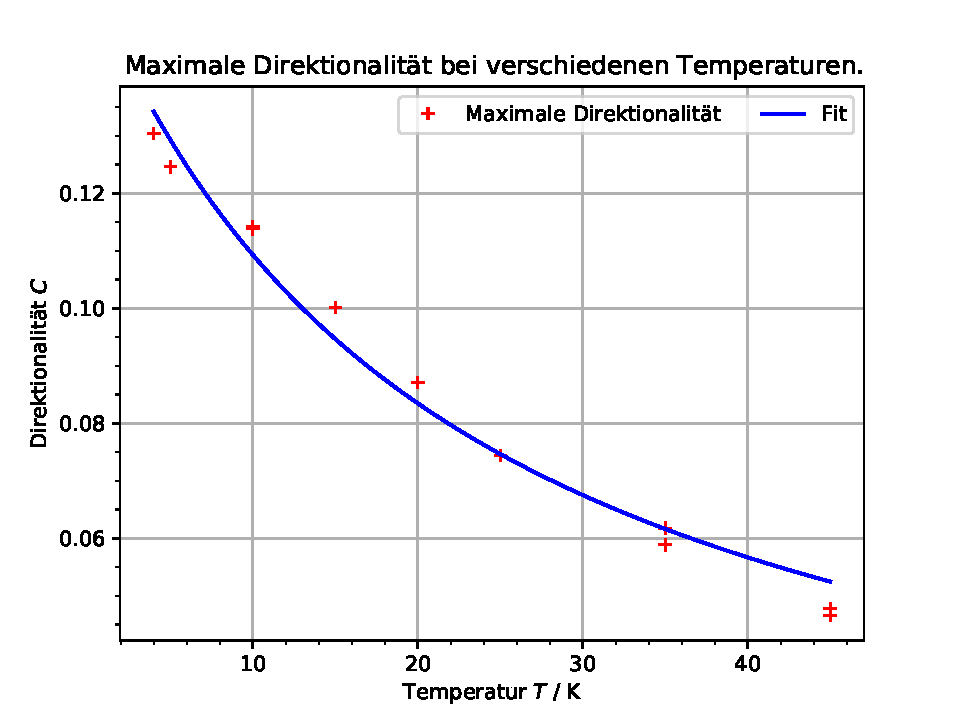
\includegraphics[scale=0.7]{./Plots/Maximale_Rho_bei_Temperaturabhänigkeit.pdf}
    \caption{Darstellung der Maximalwerte von $C$ in Abhängigkeit der Temperatur.
    Erkennbar ist die stetige Abnahme der Direktionalität $C$ bei steigender Temperatur.}
    \label{fig:fit}
\end{figure}
\FloatBarrier

Um den ebenfalls dargestellten Fit des Graphen zu erklären
sind erweiternde theoretische Erläuterungen bezogen auf Anschnitt~\ref{sec:pl} notwendig.
Die im Abschnitt~\ref{sec:pl} verwendete Gleichung 
\begin{align*}
    P_c \approx \frac{2}{3} \frac{\Delta_\text{h,F}(T)}{\Delta_\text{lh}} \propto B
\end{align*}
gilt für den Bereich kleiner zirkularen Polarisation $P_{c}\ll 1$. 
Die Größe $\Delta_\text{h,F}(T)$ aus Gleichung~\ref{eq:pc} beschreibt die 
Zeeman-Aufspaltung der Schwerlöcher in der Faraday Geometrie.
Die Aufspaltung ist weiter definiert als 
\begin{equation}
    \Delta_\text{h,F} = xN_0\beta \bigl< S^\text{Mn}_{z} \bigr>.
\end{equation}
Dabei ist $x$ die Konzentration der $\text{Mn}^\text{2+}\text{-Ionen}$ in der Probe,
$N_0\beta = -\SI{0.88}{\eV}$ die Austauschkonstante für das Valenzband und 
$\bigl< S^\text{Mn}_{z} \bigr>$ beschreibt das thermische Mittel der Spinausrichtung
der Mn-Ionen entlang der Magnetfeldlinien des angelegten Magnetfelds.

Hierbei setzt sich $\bigl< S^\text{Mn}_{z} \bigr>$ zusammen aus 
\begin{align}
    \label{eq:S}
    \bigl< S^\text{Mn}_{z} \bigr> &= S_\text{eff} B_\text{$\frac{5}{2}$} \left(\frac{5}{2}\frac{g_\text{Mn} \mu_\text{B} B }{T_\text{eff} k_\text{B}} \right)\text{.}
    %\xi &= \frac{5}{2}\frac{g_\text{Mn} \mu_\text{B} B }{T_\text{eff} k_\text{B}}\text{,}\\
    %\label{eq:S3}
    %T_\text{eff} &= T_\text{c} + T_0\text{.} 
\end{align}
Die effektive Temperatur $T_\text{eff}$ ist die Summe der Temperaturen $T_0$ und $T_\text{c}$.
Die Temperatur $T_\text{c}$
steht für die Temperatur des Atomgitters und $T_0$ beschreibt einen Offset welcher durch Antiferromagnetische Eigenschaften
von Mn-Paaren entsteht. Vorhergehende Experimente liefern hier einen Wert von $T_0=\SI{2}{\kelvin}$.
Die Funktion $B_{S}$ in Gleichung~\ref{eq:S} ist die Brillouin-Funktion 
\begin{equation}
    B_{S}(\xi) = \frac{2S+1}{2S}\coth\left(\frac{2S+1}{2S}\xi\right) - \frac{1}{2S}\coth(\frac{1}{2S}\xi),
\end{equation}
mit der Spinquantenzahl von $ S = \frac{5}{2}$~\cite{felix}.
Die Größe $g_\text{Mn} = 2 $ ist der Landé-Faktor, $\mu_\text{B}$ das Bohrsche Magneton,
$k_\text{B}$ die Boltzmann-Konstante, $S_\text{eff}$ den effektiven Spin und $B=\SI{0,5}{\tesla} $ das angelegte Magnetfeld.

Gleichung~\ref{eq:S} lässt sich jetzt in folgende Gleichung überführen
\begin{align}
    C(T)&= C_0 B_\text{$\frac{5}{2}$} (\xi)\text{,} \\
    \xi &= \frac{5}{2}\frac{g_\text{Mn} \mu_\text{B} B }{T^*_\text{eff} k_\text{B}}\text{,} \\
    T^*_\text{eff} &= T + T_0 + T_\text{off}\text{.}
\end{align}
Hierbei ist $C(T)$ jetzt auch die Funktion die für den Fit in Abbildung~\ref{fig:fit} benutzt wird.
Es gilt folgende Proportionalität
\begin{equation}
    P_{c} \propto \bigl< S^\text{Mn}_{z} \bigr> \propto C(T)
\end{equation}
Die Proportionalität trifft also eine Aussage welchen Einfluss der Grad der zirkularen Polarisation $P_{c}$
auf die Direktionalität $C(T)$ hat. 
Je größer $P_{c}$ desto größer wird die messbare Direktionalität sein. 
Hauptaugenmerk ist die Temperaturabhängigkeit von $C(T)$, diese beeinflusst $P_{c}$.
Diese besteht im einzelnen aus 
einer modifizierten effektiven Temperatur $T^*_\text{eff}$, die aus der Summe von der gemessen Temperatur $T$, dem 
Offset $T_0$ durch die Mn-Paare (siehe oben)  und dem Offset $T_\text{off}$ welches
die Temperaturdifferenz zwischen der Temperatur des Sensors und der im Experiment gemessenen entspricht. 
Die Differenz kommt dadurch zustande, dass sich die Probe nicht in einen Bad aus flüssigem Helium befindet
und der Temperatursensor nicht direkt auf der Probe angebracht ist, sondern etwas weiter entfernt. 
Die Fitparameter sind $C_0$ und $T_\text{off}$ liefern Auswertung die Werte 
\begin{align}
    C_0 & = 4.3 ± 0.2, \\
    T_\text{off} & = \SI{ 23 \pm 2}{\kelvin}. 
\end{align}
Das Temperatur Offset hat mit $T_\text{off} = \SI{ 23 \pm 2}{\kelvin}$ einen sehr hohen Wert
im Vergleich zu der gemessenen Temperaturen $T$.
Dieser Wert kann durch die Energiedichte des verwendeten Lasers von $\SI{400}{\watt\per\centi\meter^{-2}}$
erklärt werden.
Der Lasers verursacht im QW an mehreren Stellen kleine lokale Temperaturerhöhungen welche nicht 
von Temperatursensor erfasst werden können.
Effektiv ist aber auch am Graph zu erkennen, dass eine Temperaturabhängig der Direktionalität
vorhanden ist.
Die Direktionalität sinkt mit steigender Temperatur.
Anschaulich ist das auf die erschwerte Spinausrichtung der Mn-Atome im Magnetfeld zurückzuführen.

